% Created by tikzDevice version 0.9 on 2016-02-01 20:49:53
% !TEX encoding = UTF-8 Unicode
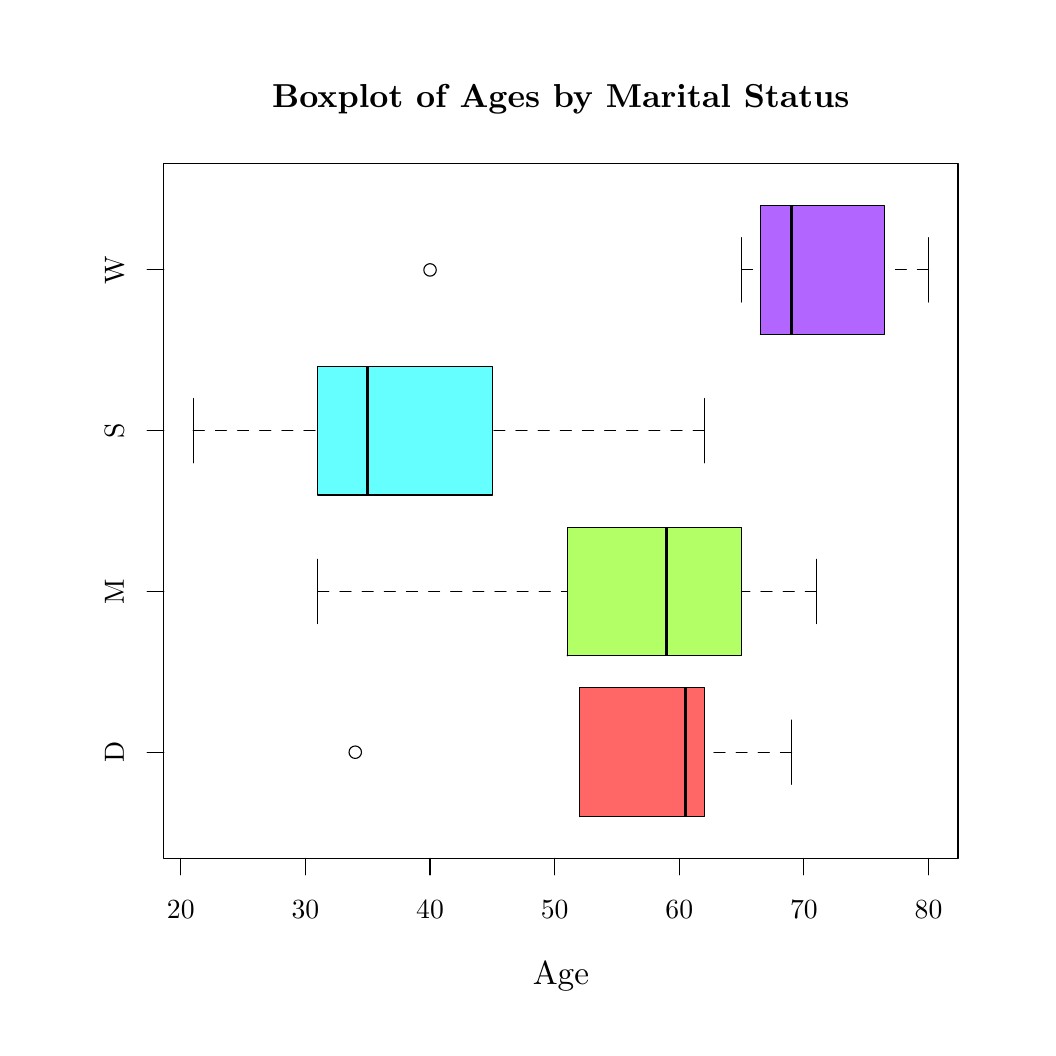
\begin{tikzpicture}[x=1pt,y=1pt]
\definecolor{fillColor}{RGB}{255,255,255}
\path[use as bounding box,fill=fillColor,fill opacity=0.00] (0,0) rectangle (361.35,361.35);
\begin{scope}
\path[clip] ( 49.20, 61.20) rectangle (336.15,312.15);
\definecolor{fillColor}{RGB}{255,102,102}

\path[fill=fillColor] (199.43, 76.30) --
	(199.43,122.78) --
	(244.46,122.78) --
	(244.46, 76.30) --
	cycle;
\definecolor{drawColor}{RGB}{0,0,0}

\path[draw=drawColor,line width= 1.2pt,line join=round] (237.71, 76.30) -- (237.71,122.78);

\path[draw=drawColor,line width= 0.4pt,dash pattern=on 4pt off 4pt ,line join=round,line cap=round] (199.43, 99.54) -- (199.43, 99.54);

\path[draw=drawColor,line width= 0.4pt,dash pattern=on 4pt off 4pt ,line join=round,line cap=round] (275.99, 99.54) -- (244.46, 99.54);

\path[draw=drawColor,line width= 0.4pt,line join=round,line cap=round] (199.43, 87.92) -- (199.43,111.16);

\path[draw=drawColor,line width= 0.4pt,line join=round,line cap=round] (275.99, 87.92) -- (275.99,111.16);

\path[draw=drawColor,line width= 0.4pt,line join=round,line cap=round] (199.43, 76.30) --
	(199.43,122.78) --
	(244.46,122.78) --
	(244.46, 76.30) --
	(199.43, 76.30);

\path[draw=drawColor,line width= 0.4pt,line join=round,line cap=round] (118.37, 99.54) circle (  2.25);
\definecolor{fillColor}{RGB}{179,255,102}

\path[fill=fillColor] (194.93,134.39) --
	(194.93,180.87) --
	(257.97,180.87) --
	(257.97,134.39) --
	cycle;

\path[draw=drawColor,line width= 1.2pt,line join=round] (230.95,134.39) -- (230.95,180.87);

\path[draw=drawColor,line width= 0.4pt,dash pattern=on 4pt off 4pt ,line join=round,line cap=round] (104.86,157.63) -- (194.93,157.63);

\path[draw=drawColor,line width= 0.4pt,dash pattern=on 4pt off 4pt ,line join=round,line cap=round] (284.99,157.63) -- (257.97,157.63);

\path[draw=drawColor,line width= 0.4pt,line join=round,line cap=round] (104.86,146.01) -- (104.86,169.25);

\path[draw=drawColor,line width= 0.4pt,line join=round,line cap=round] (284.99,146.01) -- (284.99,169.25);

\path[draw=drawColor,line width= 0.4pt,line join=round,line cap=round] (194.93,134.39) --
	(194.93,180.87) --
	(257.97,180.87) --
	(257.97,134.39) --
	(194.93,134.39);
\definecolor{fillColor}{RGB}{102,255,255}

\path[fill=fillColor] (104.86,192.48) --
	(104.86,238.96) --
	(167.91,238.96) --
	(167.91,192.48) --
	cycle;

\path[draw=drawColor,line width= 1.2pt,line join=round] (122.87,192.48) -- (122.87,238.96);

\path[draw=drawColor,line width= 0.4pt,dash pattern=on 4pt off 4pt ,line join=round,line cap=round] ( 59.83,215.72) -- (104.86,215.72);

\path[draw=drawColor,line width= 0.4pt,dash pattern=on 4pt off 4pt ,line join=round,line cap=round] (244.46,215.72) -- (167.91,215.72);

\path[draw=drawColor,line width= 0.4pt,line join=round,line cap=round] ( 59.83,204.10) -- ( 59.83,227.34);

\path[draw=drawColor,line width= 0.4pt,line join=round,line cap=round] (244.46,204.10) -- (244.46,227.34);

\path[draw=drawColor,line width= 0.4pt,line join=round,line cap=round] (104.86,192.48) --
	(104.86,238.96) --
	(167.91,238.96) --
	(167.91,192.48) --
	(104.86,192.48);
\definecolor{fillColor}{RGB}{179,102,255}

\path[fill=fillColor] (264.73,250.57) --
	(264.73,297.05) --
	(309.76,297.05) --
	(309.76,250.57) --
	cycle;

\path[draw=drawColor,line width= 1.2pt,line join=round] (275.99,250.57) -- (275.99,297.05);

\path[draw=drawColor,line width= 0.4pt,dash pattern=on 4pt off 4pt ,line join=round,line cap=round] (257.97,273.81) -- (264.73,273.81);

\path[draw=drawColor,line width= 0.4pt,dash pattern=on 4pt off 4pt ,line join=round,line cap=round] (325.52,273.81) -- (309.76,273.81);

\path[draw=drawColor,line width= 0.4pt,line join=round,line cap=round] (257.97,262.19) -- (257.97,285.43);

\path[draw=drawColor,line width= 0.4pt,line join=round,line cap=round] (325.52,262.19) -- (325.52,285.43);

\path[draw=drawColor,line width= 0.4pt,line join=round,line cap=round] (264.73,250.57) --
	(264.73,297.05) --
	(309.76,297.05) --
	(309.76,250.57) --
	(264.73,250.57);

\path[draw=drawColor,line width= 0.4pt,line join=round,line cap=round] (145.39,273.81) circle (  2.25);
\end{scope}
\begin{scope}
\path[clip] (  0.00,  0.00) rectangle (361.35,361.35);
\definecolor{drawColor}{RGB}{0,0,0}

\path[draw=drawColor,line width= 0.4pt,line join=round,line cap=round] ( 49.20, 99.54) -- ( 49.20,273.81);

\path[draw=drawColor,line width= 0.4pt,line join=round,line cap=round] ( 49.20, 99.54) -- ( 43.20, 99.54);

\path[draw=drawColor,line width= 0.4pt,line join=round,line cap=round] ( 49.20,157.63) -- ( 43.20,157.63);

\path[draw=drawColor,line width= 0.4pt,line join=round,line cap=round] ( 49.20,215.72) -- ( 43.20,215.72);

\path[draw=drawColor,line width= 0.4pt,line join=round,line cap=round] ( 49.20,273.81) -- ( 43.20,273.81);

\node[text=drawColor,rotate= 90.00,anchor=base,inner sep=0pt, outer sep=0pt, scale=  1.00] at ( 34.80, 99.54) {D};

\node[text=drawColor,rotate= 90.00,anchor=base,inner sep=0pt, outer sep=0pt, scale=  1.00] at ( 34.80,157.63) {M};

\node[text=drawColor,rotate= 90.00,anchor=base,inner sep=0pt, outer sep=0pt, scale=  1.00] at ( 34.80,215.72) {S};

\node[text=drawColor,rotate= 90.00,anchor=base,inner sep=0pt, outer sep=0pt, scale=  1.00] at ( 34.80,273.81) {W};

\path[draw=drawColor,line width= 0.4pt,line join=round,line cap=round] ( 55.32, 61.20) -- (325.52, 61.20);

\path[draw=drawColor,line width= 0.4pt,line join=round,line cap=round] ( 55.32, 61.20) -- ( 55.32, 55.20);

\path[draw=drawColor,line width= 0.4pt,line join=round,line cap=round] (100.36, 61.20) -- (100.36, 55.20);

\path[draw=drawColor,line width= 0.4pt,line join=round,line cap=round] (145.39, 61.20) -- (145.39, 55.20);

\path[draw=drawColor,line width= 0.4pt,line join=round,line cap=round] (190.42, 61.20) -- (190.42, 55.20);

\path[draw=drawColor,line width= 0.4pt,line join=round,line cap=round] (235.46, 61.20) -- (235.46, 55.20);

\path[draw=drawColor,line width= 0.4pt,line join=round,line cap=round] (280.49, 61.20) -- (280.49, 55.20);

\path[draw=drawColor,line width= 0.4pt,line join=round,line cap=round] (325.52, 61.20) -- (325.52, 55.20);

\node[text=drawColor,anchor=base,inner sep=0pt, outer sep=0pt, scale=  1.00] at ( 55.32, 39.60) {20};

\node[text=drawColor,anchor=base,inner sep=0pt, outer sep=0pt, scale=  1.00] at (100.36, 39.60) {30};

\node[text=drawColor,anchor=base,inner sep=0pt, outer sep=0pt, scale=  1.00] at (145.39, 39.60) {40};

\node[text=drawColor,anchor=base,inner sep=0pt, outer sep=0pt, scale=  1.00] at (190.42, 39.60) {50};

\node[text=drawColor,anchor=base,inner sep=0pt, outer sep=0pt, scale=  1.00] at (235.46, 39.60) {60};

\node[text=drawColor,anchor=base,inner sep=0pt, outer sep=0pt, scale=  1.00] at (280.49, 39.60) {70};

\node[text=drawColor,anchor=base,inner sep=0pt, outer sep=0pt, scale=  1.00] at (325.52, 39.60) {80};
\end{scope}
\begin{scope}
\path[clip] (  0.00,  0.00) rectangle (361.35,361.35);
\definecolor{drawColor}{RGB}{0,0,0}

\node[text=drawColor,anchor=base,inner sep=0pt, outer sep=0pt, scale=  1.20] at (192.68,332.61) {\bfseries Boxplot of Ages by Marital Status};

\node[text=drawColor,anchor=base,inner sep=0pt, outer sep=0pt, scale=  1.20] at (192.68, 15.60) {Age};
\end{scope}
\begin{scope}
\path[clip] (  0.00,  0.00) rectangle (361.35,361.35);
\definecolor{drawColor}{RGB}{0,0,0}

\path[draw=drawColor,line width= 0.4pt,line join=round,line cap=round] ( 49.20, 61.20) --
	(336.15, 61.20) --
	(336.15,312.15) --
	( 49.20,312.15) --
	( 49.20, 61.20);
\end{scope}
\end{tikzpicture}
